\documentclass[12pt]{article}
\usepackage[english]{babel}
\usepackage[utf8]{inputenc}
\usepackage{fancyhdr}
\usepackage{hyperref}
\usepackage{mathrsfs}
\usepackage{amsmath}
\usepackage{graphicx}
\usepackage{pgfplots}
\pgfplotsset{width=10cm,compat=1.9}

\graphicspath{ {./images/} }

\pagestyle{fancy}
\fancyhf{}

\newcommand{\partcontent}{}
\rhead{\partcontent}
\chead{ENGR 455}
\lhead{Greg Birge}
\rfoot{Page \thepage}
\urlstyle{same}


\begin{document}
\part*{Week I}
\renewcommand\partcontent{Week I}
\section{Vectors and Vector Space Coordinates}
A useful field of mathematics for signal analysis are vectors and  vector spaces. Using models with vectors will allow for simplifying and evaluating difficult problems and forming critical theorems for technological advancements.\\

\subsection{Vector Notation}
In this notebook, vectors will be denoted by the over line, for example the vector $v$ will be denoted by  $\overline{v}$. Unit vectors to denote coordinates will be denoted by the hat, for example the unit vector j will appear as $\widehat{j}$ and unless otherwise denoted the cartesian coordinates used will be \textit{i}, \textit{j}, and \textit{k}. Dot products will be denoted by the thick dot symbold $\bullet$ and the $\cdot$ symbol will denote traditional multiplication operations.


\subsection{Orthogonal vs Orthonormal}
There is a critical difference between sets of vectors that are orthogonal and orthonormal. \textbf{Orthogonal} vectors are two or more vectors that are perpendicular to each other. \textbf{Orthonormal} vectors are orthogonal vectors with the added restriction that the vectors are unit vectors. $$\mid \widehat{i} \mid = 1$$ Orthogonal unit vectors are orthonormal. To prove orthogonality, $$\overline{u}\bullet\overline{v} = 0$$ and for orthonormality $$\Vert \overline{u} \Vert = \Vert \overline{v} \Vert$$

%\section{Change of coordinate systems}
%A common 'trick' implemented in %difficult problems and derivations is to change the coordinate system to better fit the situation. For this method we will propose a two dimensional vector $\widehat{v} = v_x\widehat{i} + v_y\widehat{j}$, where $v_x$ and $v_y$ are some scalar. We want to rewrite $\widehat{v}$ to be in terms of the orthonormal pair of vectors $\widehat{i}'$ and $\widehat{j}'$, which are defined as $$\widehat{i}' = I_x\widehat{i} + I_y\widehat{j}$$ $$\widehat{j}' = J_x\widehat{i} + J_y\widehat{j}$$ $$I_x = (\widehat{i}'\cdot\widehat{i})\quad  I_y =(\widehat{i}' \cdot \widehat{j})$$ $$J_x = (\widehat{j}' \cdot \widehat{i})\quad  J_y =(\widehat{j}' \cdot \widehat{j})$$ 

%Now with our system set up, we can rewrite $\widehat{v}$ as $\widehat{v'}$ in terms of $\widehat{i'} $ and $ \widehat{j'}$. To do this we will take the dot product of $\widehat{v}$ with the new axes defined above. $$ \widehat{v'_x} = \widehat{v} \cdot \widehat{i'} = I_x v_x + I_y v_y$$ $$\widehat{v'_y} = \widehat{v} \cdot \widehat{j'} = J_x v_x + J_y v_y$$
%Due to the new set of basis vectors being orthogonal unit vectors, $I_y = J_x = 0$, further simplifying the new prime vectors. Therefore this allows us to represent $\widehat{v}$ in terms of the new basis vectors, giving us: $$\widehat{v'} = I_x v_x \widehat{i'} + J_y v_y \widehat{j'} $$ 
%An important thing to note about the above derivation, is that it depends on the new axes being an orthonormal pair. Generally new reference axes will be mapped to orthogonal sets of vectors yet they won't always be orthonormal.

\subsection{N-dimensional coordinate change}
In signal analysis, changing coordinate systems for $N$ dimensions is a common problem. In addition to this, we often don't require the entire matrix and might only need one new component. Suppose we have some vector $\widehat{v}$ of length $N$ and we want a new vector in terms of $\widehat{k'}$. This component can be calculated using a dot product with the $N$ by $N$ transformation matrix and simplified into a single summation. $$\widehat{v'_n} = \frac{1}{\mid \widehat{k'} \mid ^2} \cdot \sum_{i=0}^{N} (k_{n,i} \cdot v_i) $$

A modified version of the above equation forms the basis of a critical tool to signal analysis, the Fourier Transform. The different forms will be explored in weeks to come but we will go over the change needed to be made. With $\widehat{k'}$ and $\widehat{n}$ defined as $\widehat{k'} \bullet \widehat{n}= \mid\widehat{n}\mid^2\delta_{k'n}$, we can replace: $$\mid\widehat{n}\mid^2\delta_{k'n} = e^\frac{2 \pi jnk}{N}$$ Therefore, $\widehat{v} \bullet \widehat{n} $ can be rewritten as $$\widehat{v} \cdot \widehat{n} = \sum_k^N v_k e^\frac{2 \pi jnk}{N}$$
\noindent\makebox[\linewidth]{\rule{\paperwidth}{0.4pt}}


\part*{Week II}
\renewcommand\partcontent{Week II}
\section{Introduction to Fourier Series}
For a proper introduction, let us begin by looking at the below waveform. This waveform looks ugly and could be difficult to model. However, this waveform was easily generated using adding together two sine waves together, those functions having their graphs shown below.\\
\begin{tikzpicture}
\begin{axis}[
	axis lines = left,
	domain = 0:2*pi,
	samples=100,
	no marks,
	xtick={0,6.2832},
	xticklabels={0,2$\pi$},	
	x post scale=1,
	y post scale=0.85
]
\addplot {2*sin(deg(x))+0.8*sin(3*deg(x) - 4))};
\end{axis}
\end{tikzpicture} % 
\\
\begin{tikzpicture}
\begin{axis}[
	axis lines = left,
	domain = 0:2*pi,
	samples=200,
	no marks,
	xtick={0,6.2832},
	xticklabels={0,2$\pi$},
	x post scale=1,
	y post scale=0.85
]
\addplot {2*sin(deg(x))};
\addplot [color=red]{0.8*sin(3*deg(x) - 4))};
\end{axis}
\end{tikzpicture}

The guiding principal of Fourier series is this aspect, multiple sine waves of varying magnitudes and angles making up the component parts of a waveform. Notice that the top graph has two different peaks that coincide with the lining up of the peak amplitudes of the red and blue graphs. Joseph Fourier initially used this method to approximate the step function as seen in the heat transfer problem of connecting a hot rod to a cold rod in physics$^1$. He used these series of sine waves to add up and approximate closer and closer to square waves. His work has found its place in many other applications and fields$^1$. It is a critical concept for modern day digital signal processing and frequency analysis.

Before we begin, further background information is necessary. Primarily that we will be representing the sine waves as vectors on the real and imaginary coordinate plane. This is done using Euler's Formula $$ e^{j \phi} = cos(\phi) + jsin(\phi)$$ His formula allows us to show a vector in this complex plane with a magnitude $A$ and angle $\theta$ as $Ae^{j\theta}$. This greatly simplifies the math needed for working with Fourier Series. For reference here is the Fourier Series in the time domain missing this simplification. $$f(t) = 0.5a_0 + \sum_{k=1}^{\infty}(a_kcos(2\pi kt) + b_ksin(2 \pi kt))$$

%Maybe show none euler's identity derivation
Using Euler's identity, we can derive the following series with $c_n$ as the vector magnitude and $e^{j\pi t}$ the angle with respect to time. Our $e^{j\pi t}$ term will also have an $n$ term to keep track of which vector in the Fourier series we are looking at. Whether that is the $n=1$ vector or the $n=20$ or higher vector. $T_0$ is the period over which we examining this Fourier Series.
$$ f(t) = \sum_{n=-\infty}^{\infty} c_n e^{\frac{j\pi nt}{T_0}} $$ 

We will explore the method to solve for the coefficients $c_n$ in a later notebook.

\subsection{Dirac Delta Function}
To better understand some parts in later derivations, we need to define what is known as the Dirac delta function $\delta(t)$ also known as the Impulse function. It is unique for it is only equal to 1 at a single point such that one with no translation would be: $$ \delta (x) = \begin{cases} 
      0 & x \neq 0 \\
      \infty & x = 0 \\
   \end{cases} $$ Or for definition's sake, a Dirac delta shifted over $u$ along the x-axis: $$ \delta (x-u) = \begin{cases} 
      0 & x \neq 0 \\
      \infty & x = u \\
   \end{cases} $$
   
The Dirac delta is also known as the 'Sifting Function,' for its commonly known sifting property where across an infinite domain, it will return only the value at one point. For any function $f(x)$: $$ \int_{-\infty}^{\infty} f(x) \cdot \delta(x-a)dx = f(a) $$ 
The Dirac delta's sifting property will prove to be very useful in the next section. 
 $$\rightarrow \int_{-\infty}^{\infty} e^{-j2\pi fu} \cdot e^{j2\pi ft} df $$ 
 $$ \rightarrow \int_{-\infty}^{\infty} e^{(t-u)j2\pi f} df $$ $$ \rightarrow \frac{e^{(t-u)j2\pi f}}{j2\pi (t-u)} \bigg\rvert_{-\infty}^{\infty} $$ This integral only has a valid answer when $t=u$, therefore it has the same value as a delta function. This gives the helpful identity: $$\Rightarrow \int_{-\infty}^{\infty} e^{-j2\pi fu} \cdot e^{j2\pi ft} df = \delta_{tu}(f) $$

\subsection{Discrete Fourier Transform Derivation}
 The Discrete Fourier Series is simply the above equation in a discrete range. That series would be very useful to us if we could transform a periodic function in the time domain into the frequency domain as a Fourier series. This is done using the Discrete Fourier Transform (DFT). Leaving the definition of the DFT as just the discretized Fourier Transform would be ignorant of its roots in vector math and how viewing its derivation through vectors better simplifies the mathematics of the process. Relating this to the definition provided above, it is seen that the Fourier transform allows one to determine the magnitude and angle of a component sinusoidal equation in a line. These sine waves correspond to vectors in the complex+real plane, hence, a Fourier transform can be seen as finding the component vector in the desired direction. A dot product of a vector $\widehat{a}$ and unit vector $\widehat{b'}$ yields the vector component of $\hat{a}$ in the direction of $\widehat{b'}$. The derivation below shows how these dot products lead to the DFT. For this example, let us have a vector $\widehat{v}$ with components in the $\widehat{k}$ and $\widehat{n'}$ directions. \textit{Note: $\bar{A} \cdot \bar{B} = (\bar{B} \cdot \bar{A})^*$, with $^*$ denoting the complex conjugate.} \textit{Also, the $\bullet$ symbol will be used to signify Dot products while $\cdot$ will be for multiplication operations. } $$\widehat{v} = \sum_{k=0}^{N-1} v_k \widehat{k} = \sum_{n'=0}^{N-1} v'_{n'} \widehat{n'} $$
 With this we need the component of $\hat{v}$ in the $\widehat{m'}$ direction: $$\rightarrow \hat{v} \bullet \widehat{m'} = \sum_{k=0}^{N-1} v_k \widehat{k} \bullet \widehat{m'} = \sum_{n'=0}^{N-1}v'_{n'} \widehat{n'} \bullet \widehat{m'}  $$ $$\rightarrow \sum_{k=0}^{N-1} v_k \widehat{k} \cdot \widehat{m'} = \sum_{n'=0}^{N-1} v'_{n'} |\widehat{m'}|^2 \delta_{n'm'}$$
 $$\rightarrow \sum_{k=0}^{N-1} v_k \widehat{k} \cdot \widehat{m'} = v'_{m'} |\widehat{m'}|^2 $$ $$ \rightarrow v'_{m'} = \sum_{k=0}^{N-1} v_k \frac {\widehat{k} \cdot \widehat{m'} }{|\widehat{m'}|^2} $$
 We can define $\frac {\widehat{m'} \cdot \widehat{k} }{|\widehat{m'}|^2}$ as $e^{j2\pi m'k/N}$ because we are wanting to change the coordinate system akin to Euler's identity above. With this in mind, we can replace it with its complex conjugate. Giving us the Discrete Fourier Transform below. $$\rightarrow v'_{m'} = \sum_{k=0}^{N-1} v_k e^{-j2\pi m'k/N} $$
This shows just how the DFT is really a special case of a change of basis coordinates between the $\widehat{k}$ and $\widehat{m}$.


\subsection{Discrete Transform and Inverse Transform}
To contextualize these definitions in their applications, we will use the example of some signal, $x(t)$, sampled by an A/D converter at intervals of T seconds so that $t \in {0, T, 2T, ..., (N-1)T}$. We want the $l$'th element from the data which we would get from doing $x(lT)$ which we will define as $x(k)$, ($k = lT$). Hence we can get the Fourier Transform of our data as $X(n)$. $$n \in {0,1,,2,...., N-1}$$ $$ X(n) =  \sum_{k=0}^{N-1} x(k)e^{-j2\pi nk/N} $$ If we need to return out transformed sample data back into the time domain, we can easily find the inverse transform. We can dot product both sides using an orthogonal complex conjugate of $e^{-j2\pi nk/N}$, that conjugate being $e^{j2\pi nm/N}$, the $m$ and $k$ act as dummy variables for the sigmas, and are only different for legibility. 
$$\sum_{n=0}^{N-1}X(n)e^{j2\pi nm/N} = \sum_{k=0}^{N-1} x(k) \sum_{n=0}^{N-1} e^{-j2\pi nk/N}e^{j2\pi nm/N}  $$ The dot product of $e^{-j2\pi nk/N}$ and $e^{j2\pi nm/N}$ is only not zero where $k=m$, meaining it is effectively a $\delta$ function of $k$ and $m$. When this is true, each term is equal to 1 for $N$ terms giving us $N \delta_{km}$. $$\sum_{n=0}^{N-1}X(n)e^{j2\pi nm/N} =  \sum_{k=0}^{N-1} x(k) N \delta_{km} $$ $$ x(k) N = \sum_{n=0}^{N-1}X(n)e^{j2\pi nm/N} $$
Switching the $m$ back to a $k$ for consistency as they are just dummy variables for the sigma notation.
$$x(k) = \frac{1}{N} \sum_{k=0}^{N-1} X(n) e^{j2\pi nk/N}$$ Note that the inverse transform, save for the division by N, is merely another dot product of the $X(n)$ and the complex conjugate of $e^{-j2\pi nk/N}$. 
 
\subsubsection*{Resources} 
$^1$ \url{https://youtu.be/r6sGWTCMz2k} \\ 
%
$^2$ \url{https://youtu.be/mkGsMWi_j4Q} \\
$^3$ \url{http://fweb.wallawalla.edu/~frohro/ClassHandouts/Signals/Vectors%20and%20the%20DFT%20(early%20Work).html} \\
%
 
 
 
\noindent\makebox[\linewidth]{\rule{\paperwidth}{0.4pt}}
\part*{Week III}
\renewcommand\partcontent{Week III}
\section{Coefficients of Complex Fourier Series}
In the previous section, we derived and discussed the discrete complex Fourier series for a periodic function $x(t)$ with period $T_0$ : $$x(t) = \sum_{n = -\infty}^{\infty} c_n e^{j2\pi nt/T_0} $$ Yet we did not give a formula for finding the $c_n$ value. Viewing the Fourier series as the sum of component sine waves, represented as complex vectors, in any line, the $c_n$ can be viewed as the magnitude of the $nth$ vector in the $nth$ dimension. This contextualizes $c_n$ yet does not assist in finding its value for any equation. The below derivation tackles this issue, by looking at the relationship of $c_n$ in a periodic function where $x(t) = x(t+T_0)$, (where $T_0$ is the length of one period). 
$$ x(t) = x(t+T_0) = \sum_{n=-\infty}^{\infty} c_n e^{2\pi jnt/T_0} $$ Taking the dot product of both sides of the complex conjugate $e^{-2\pi jmt/T_0} $, where $m$ is a new dummy variable to index for the summation. \textit{Note: The $\bullet$ symbol will be used to signify Dot products while $\cdot$ will be for multiplication operations. } $$ \overline{x}(t) \bullet ( e^{-2\pi jmt/T_0}) = (\sum_{n=-\infty}^{\infty} c_n e^{2\pi jnt/T_0}) \bullet e^{-2\pi jmt/T_0} $$ 
$$\overline{x}(t) \bullet (e^{\frac{-2\pi jmt}{T_0}})  = \sum_{n=-\infty}^{\infty} \sum_{t=-\infty}^{\infty} c_n e^{2\pi jnt/T_0} e^{-2\pi jmt/T_0} $$ Taking a small aside to show what happens to the right half of this equation, looking at the portion right of $\sum\limits_{n=-\infty}^{\infty} c_n $: 
$$\rightarrow \sum_{t=-\infty}^{\infty} e^{2\pi jnt/T_0} e^{-2\pi jmt/T_0} $$
 $$\rightarrow \int_{-\infty}^{\infty} e^{2\pi jnt/T_0} e^{-2\pi jmt/T_0} dt $$ If $n \neq m$: $$ \Rightarrow \int_{-\infty}^{\infty} e^{2\pi jnt/T_0} e^{-2\pi jmt/T_0} dt = 0 $$ If $n = m$: $$\Rightarrow \int_{-\infty}^{\infty} e^{2\pi jnt/T_0} e^{-2\pi jmt/T_0} dt = T_0$$ Therefore this right summation from earlier can be replaced with a Dirac delta function for $n$ and $m$. Back to the derivative, we can begin simplifying and solving for $c_n$. $$ \overline{x}(t) \bullet (e^{-2\pi jmt/T_0})  = \sum_{n=-\infty}^{\infty} c_n T_0 \delta_{nm} $$ By nature of the Dirac delta function, we can remove the sigma on the right and begin expanding the terms on the left. $$\int_{-\infty}^{\infty} x(t)e^{-2\pi jmt/T_0}dt = c_n T_0 $$ The sigma only matters for when $n=m$, which in this case would only be within the period from 0 to $T_0$ $$\Rightarrow c_n = 1/T_0  \int_{-\infty}^{\infty} x(t)e^{-2\pi jn/T_0} dt$$ %maybe put an equation number here like (3.1)
\\
The last notable property of the $c_n$ constants are how they behave when in the real domain. For the above equation, if $x(t) \in \Re$ then the constants $c_n = c_{-n}^* $

\subsection{Fourier Transforms}
Fourier series will be most useful to us if we can accurately apply it to a non periodic function. For this we will look at some waveform defined as $x(t)$ and another point at $x(t+T_0)$ such that $x(t) = x(t+T_0)$. However, in this case we are not assuming the function is periodic, merely that there are two different points along the $t$ axis where they are equivalent. Shown here equal to its complex Fourier series. $$x(t) = x(t+T_0) = \sum_{n=-\infty}^{\infty} c_n \cdot e^{-2\pi jnt/T_0}$$ We will sub in the definition of $c_n$ however as a continuous summation (integral) from $-T_0/2$ to $T_0/2$ and with x(t) written with a different dummy variable $u$: $$ x(t) = \frac{1}{T_0} \sum_{n=-\infty}^{\infty}e^{2\pi jnt/T_0} \int_{-T_0/2}^{T_0/2} x(u)e^{-2\pi jnu/T_0} du $$ With the equation in this form, we can make a critical change of variables. Note that in both complex exponentials there is a $\frac{n}{T_0}$ term. $\frac{n}{T_0}$ is in units of inverse seconds as the $n$ lacks units, meaning we can easily change this term to $f$ to stand for frequency, as that is what it effectively is. The $n'th$ frequency across $T_0$ would occur at $T_0$.
$$ x(t) = \frac{1}{T_0} \sum_{n=-\infty}^{\infty}e^{2\pi jtf} \int_{-T_0/2}^{T_0/2} x(u)e^{-2\pi juf} du $$

Therefore with this substitution in mind, we also will take the limit of both sides as $T_0$ approaches infinity. Doing this will turn the $\frac{1}{T_0}$ term into a term along the $f$ axis that is infinitely small and evenly spaced apart, $df$. This also allows us to replace the sigma with an integral: $$\lim_{T_0\to\infty} x(t) = \lim_{T_0\to\infty} \frac{1}{T_0} \sum_{n=-\infty}^{\infty}e^{2\pi jtf} \int_{-T_0/2}^{T_0/2} x(u)e^{-2\pi juf} du $$ $$\rightarrow x(t) = \int_{-\infty}^{\infty}e^{2\pi jtf} [\int_{-\infty}^{\infty} x(u)e^{-2\pi juf} du] df $$ 
Taking a step back from this equation, it seems we have just derived both the Fourier Transform and Inverse Fourier transform. Looking at the equation right now, you will see that in the inner integral from $[-T_0/2:T_0/2]$ takes a function of some variable $u$ (which could be replaced with $t$) into the $f$ domain. And the same goes for the outer integral from ($-\infty:\infty$) returning the equation in the $f$ domain back to the time domain. Giving us the transforms denoted by the script F $\rightarrow \mathscr{F}$. \\
Fourier Transform: $$\Rightarrow X(f) = \mathscr{F}[x(t)] = \int_{-\infty}^{\infty} x(t)e^{-2\pi jtf} du $$ Inverse Fourier Transform: $$\Rightarrow x(t) = \mathscr{F}^{-1}[X(f)] = \int_{-\infty}^{\infty}e^{2\pi jtf} X(f) df$$  	

\noindent\makebox[\linewidth]{\rule{\paperwidth}{0.4pt}}

\part*{Week IV}
\renewcommand\partcontent{Week IV}
\section{Intro to Systems}
So far in these notebooks, we have primarily focused on analyzing signals. These signals will serve as being the inputs and generally the outputs of our systems. However, we need to start taking a closer look at the type of systems we will be working with. A loose definition of a \textbf{system} is some collection of modules that when given a signal, generate a response in some way$^4$. \\

For this notebook, we will be focusing on one class of systems in particular, \textbf{Linear Time-Invariant Systems.} This class of systems is important to us as engineers because the math required to solve linear problems is considerably easier than nonlinear systems. Add to this that the system's response won't vary with respect to time and that is one less variable to worry about changing. For these systems, something that matters a lot to us is see how we can predict what the output will be based on what we input and the rules of the system, almost like a game.


\subsection{L.T.I. Game}
To understand the different properties of L.T.I. systems, we need to look at how different inputs to our system will generate outputs. For this game, we will refer to our system as $\mathscr{T}$. We will use $\rightarrow$  to denote a flow of data either in or out of a system. $x(t)$ will be our input signal in the time domain and generally $y(t)$ will denote the output signal. A prime example of this notation will be our first input $x(t)$. $$x(t) \rightarrow \mathscr{T} \rightarrow y(t) $$
The linearity property of the system allows us to predict many possible outputs. If there is a scalar factor on the input $x(t)$, we will see it in the output of the system: $$\alpha x(t) \rightarrow \mathscr{T} \rightarrow \alpha y(t) $$ Another principle of linear systems we can use is the \textit{principle of superposition} which states that if the input to the linear system is a sum of two or more scaled sequences, we can find the output due to each sequence acting alone and then superimpose the two scaled outputs. $$x_1(t) + x_2(t) \rightarrow \mathscr{T} \rightarrow y_1(t) + y_2(t) $$ This is the same for some factor that scales the inputs represented by $\alpha$ and $\beta$. $$\alpha x_1{t} + \beta x_2(t) \rightarrow \mathscr{T} \rightarrow \alpha y_1(t) + \beta y_2(t) $$

The \textit{time-invariant} part of our \textit{L.T.I.} system allows us to make predictions where our output will occur at the same time as our input. Even if our input has been shifted by some value, $t_0$, we know our output will be shifted and equal amount in the same direction, such that: 
$$ x(t-t_0) \rightarrow \mathscr{T} \rightarrow y(t-t_0) $$

Something that is known to us is that inputting a $\delta$ function with the sifting property will give us a set output. This known output $h(t)$, is what we will know it as the \textbf{impulse response}. $$ \delta(t) \rightarrow \mathscr{T} \rightarrow h(t) $$ Due to the time-invariant nature of the system, we also know that: $$ \delta(t-t_0) \rightarrow \mathscr{T} \rightarrow h(t-t_0) $$ 


From our earlier work with delta functions, we know that some function $x(t)$ times an impulse will equal that function at that impulse, $x(t_0)$.  $$ x(t_0) \delta (t-t_0) \rightarrow \mathscr{T} \rightarrow x(t_0) h(t-t_0) $$
We also know based on the linearity and time-invariance of the system that we can treat each impulse input as a linear sum of terms. Meaning we can add up all of those impulse inputs to get the total of our impulse responses.
$$ \int_{-\infty}^{\infty} x(t_0) \delta (t-t_0)dt \rightarrow \mathscr{T} \rightarrow \int_{-\infty}^{\infty} x(t_0) h(t-t_0)dt $$
That $y(t)$ is what is known as a convolution integral: $ x(t) * h(t) $. This convolution integral can be seen as accomplishing the same as a multiplication operation in the frequency domain but in the time domain. \\

Suppose we want to  input some signal of a specific frequency $f$ into an LTI system. This signal, $e^{j2\pi ft}$ can just be plugged in the place of our arbitrary input function $x(t)$. We can use the earlier defined behavior and apply that to our signal: $$e^{j2\pi ft_0} \delta (t-t_0) \rightarrow \mathscr{T} \rightarrow  \int_{-\infty}^{\infty} e^{j2\pi f t_0}*h(t-t_0) du $$
With a change of variables we can simplify this further predicted output even further. Setting $ u = t-t_0 $ and therefore $du = -dt_0 $ Our output becomes $$\Rightarrow - \int_{\infty}^{-\infty} e^{j2\pi f(t-u)}h(u)du$$ $$\Rightarrow e^{j2\pi ft} \int_{-\infty}^{\infty} e^{-j2\pi fu} h(u)du$$
The remaining integral is the Fourier transform of our impulse response $h(t)$. Meaning our LTI system, when given a signal with an impulse will output that signal times the Fourier transform. This should be expected as we effectively went from taking the convolution of our given exponential signal at some frequency and derived that our output would just be multiplication in the frequency domain. This is consistent with what we have discussed so far about convolution integrals. $$e^{j2\pi ft_0} \delta (t-t_0) \rightarrow \mathscr{T} \rightarrow  e^{j2\pi ft} \cdot  H(f) $$


\noindent\makebox[\linewidth]{\rule{\paperwidth}{0.4pt}}

\part*{Week V}
\renewcommand\partcontent{Week V}
\section{Intro to A/D Conversion}
Suppose you were sampling an analog input to be recorded digitally. Once those values in the time domain were recorded, to work with them efficiently, you would want to convert to the frequency domain using the Fourier Transform. However, it is a difficult continuous integral that works better the closer you can get to an infinitesimal sample rate. Wanting to simplify the amount of computation that needs to be done, an alternative method needs to be devised. Luckily, we can replace the Fourier Transform exactly, using a Discrete Fourier Transform. We want to replace the $c_n$ term using the DFT, so we will start with $c_n$ across one period $T_0$. $$c_n = \frac{1}{T_0} \int_{0}^{T_0} x(t)e^{-j2\pi nt/T_0} dt $$ We are going to take this equation and approximate it using the DFT. We are taking $N$ samples that are $T$ seconds apart, across our $T_0$ period, giving us $T_0 = NT$. $$\rightarrow \frac{1}{NT} \sum_{k=0}^{N-1} x(kT)e^{\frac{-j2\pi nkT}{NT}} \cdot T $$
$$\rightarrow \frac{1}{N} \sum_{k=0}^{N-1} x(kT)e^{\frac{-j2\pi nk}{N}}$$ 
$$\rightarrow \frac{1}{N} DFT(x(k))$$

For a practical application, an extra step needs to be taken to use this approximation. The DFT assumes the signal is periodic indefinitely and many real world samples, primarily audio signals, are not periodic. To account for this, the recorder can leave dead time before and after the sample, ensuring $x(0) = x(NT)$.

The approximation using the DFT can be made exact yet it isn't always due to the phenomena known as \textbf{aliasing}, and has much to do with the sample rate. Aliasing is when your samples look to be reading the desired signal yet in reality you are sampling too slow and there is a much higher frequency \textit{alias} signal that appears equal to ours at each sample. This is best illustrated graphically$^2$.\\ 
\includegraphics[scale=0.85]{aliasingB}
See the red signal's samples all line up with the much higher frequency blue signal. To avoid incorrectly reading high frequency signals as low frequency or vice versa, we need to know how to pick our sample rate. The \textbf{Nyquist Theorem} answers this question. The Nyquist Theorem states: \\\textit{"If a function $x(t)$ contains no frequencies higher than B hertz, it is completely determined by giving its ordinates at a series of points spaced $\frac{1}{2B}$ seconds apart."}$^4$\\
This gives us a desired sample rate of two times the desired highest frequency recorded. Following the constraint proposed by Nyquist theorem gives us a DFT that will exactly equal the sampled signal without using the Fourier transform. In  practical applications, we would need a low-pass filter to ensure that the highest frequencies present are at or below our sample rate.


\subsubsection*{Resources and Further Reading}
$^1$ \url{https://brilliant.org/wiki/signals-and-systems/} \\
$^2$ \url{http://blog.dataphysics.com/dynamic-signal-analysis-review-aliasing/} \\
$^3$ \url{https://brilliant.org/wiki/linear-time-invariant-systems/} \\
$^4$ \url{https://en.wikipedia.org/wiki/Nyquist%E2%80%93Shannon_sampling_theorem}

\noindent\makebox[\linewidth]{\rule{\paperwidth}{0.4pt}}

\part*{Week VI}
\renewcommand\partcontent{Week VI}
\section{Processing and Reconstructing a Signal}
In the last week's section, we introduced the problem presented by recording an audio signal digitally. We covered how once the constraints set by the Nyquist Theorem are met, we can accurately record any signal so long as our sample rate is fast enough and all unwanted high frequency signals are filtered out with a low pass filter. Our system follows this block diagram:\\ \includegraphics[scale=0.53]{cdRecordSys_source}
\\ Now we will cover the method used to digitally filter the recorded waveform in our system although many other methods exist. This method is known as using a \textbf{Finite Impulse Response} Filter or \textbf{FIR Filter} for short. 
\\

\subsection{FIR Filter}
Looking at the above diagram, you can see that at this point, our signal has been sampled and recorded by an A/D converter. Based on what we have covered so far, the primary thing we will do to it is to transfer it into the frequency domain. Taking the DFT of our data will give us some signal $x(t)$ in the domain $k \in (0,1T,2T,...,(N-1)T) )$ and $n$ is in the domain $n \in ({0, 1, ..., N-1}) $. $$ X(n) = DFT(x(k))$$. 
The goal of our filter depends on the application. For the given example, we would want  The FIR filter works where the desired impulse responses are solved for and multiplied to develop the output signal in the Frequency domain: $$Y_0(n) = X(n)\cdot H(n)$$
These impulse responses are determined by taking the IDFT of the responses in the frequency domain: $$h(k) = IDFT[H(n)] $$ $$ h(k) = \frac{1}{N} \sum_{m=0}^{N-1} h(m)\cdot e^{\frac{j2\pi mn}{N}} $$ If we want the output $Y_0(n)$ back into the time domain, we need to solve for it: $$y(k) = IDFT[DFT(x(k))\cdot H(n)]$$ 

$$\rightarrow	\frac{1}{N} \sum_{n=0}^{N-1} \Bigg( \sum_{l=0}^{N-1} x(l)\cdot e^{\frac{j2\pi ln}{N}} \Bigg) \cdot \Bigg( \sum_{m=0}^{N-1} h(m)\cdot e^{\frac{j2\pi mn}{N}} \Bigg) e^{\frac{j2\pi nk}{N}} $$

$$\rightarrow \frac{1}{N} \sum_{l=0}^{N-1} x(l) \sum_{m=0}^{N-1} h(m) \sum_{n=0}^{N-1} e^{\frac{j2\pi n(k-m-l)}{N}} $$

Here there are two possible values for $\sum_{n=0}^{N-1} e^{\frac{j2\pi n(k-m-l)}{N}}$ that matter for us:
$$ \rightarrow	\sum_{n=0}^{N-1} e^{\frac{j2\pi n(k-m-l)}{N}}  = N\delta_{m, k-l} = N\delta_{l,k-m} $$

For $N \cdot \delta_{m, k-l}$: 
$$\rightarrow y(k) = \sum_{l=0}^{N-1} x(l) \sum_{m=0}^{N-1} h(m) \delta_{m, k-l}$$ 
$$\rightarrow \sum_{l=0}^{N-1} x(l) h(k-l)$$ 
$$\Rightarrow y(k) = x(k) * h(k) $$

For $N \cdot \delta_{l, k-m}$: 
$$ \rightarrow y(k) = \sum_{l=0}^{N-1} x(l) \sum_{m=0}^{N-1} h(m) \delta_{l, k-m} $$
$$ \rightarrow \sum_{l=0}^{N-1} x(l) h(k-m)$$ 
$$ \Rightarrow y(k) = h(k) * x(k) $$
This $y(k)$ is our output signal in the time domain after it has been filtered to fit our desired impulse response. 
%motivation for time domain is realtime filtering
%
\subsection{Real Time Filtering}
A very useful application of signal processing is being able to filer in real time. So far, many of the filtering and processing methods we have discussed have high \textbf{latency}, which is the amount of delay between the input entering the system and an output signal/action occurring. Our previous discussed methods have latency issues because we are doing the operations in the frequency domain. To transform our data with a Fourier transform, we need to have sampled the entirety of the input signal. This creates a minimum latency as long as our sample. For example, if we were filtering the signal from a microphone for a singer, our filter will have a latency of one whole song which is very impractical.

This is why real time filtering can be very useful. The solution is to perform the filtering operations over much smaller lengths of time in the time domain. This can be done using convolutions in the time domain, which was just above proved to be equivalent to multiplication operations in the frequency domain. Convolutions in the time domain work better than having to transform to frequency is due to the number of multiplication operations needed to be completed. For $N$ samples, a fast Fourier transform (common algorithm used in place of DFT) has $N*log_{10}(N)$ operations, while time domain convolutions have $N^2$ operations. This makes sense why for larger sample sets, it is good practice to avoid working in the time domain. Yet when $N$ is very small, the difference in number of operations is very small. The processor can quickly perform its filtering over a very small sample set and deliver the output with considerably lower latency by performing convolutions in the time domain.
\\
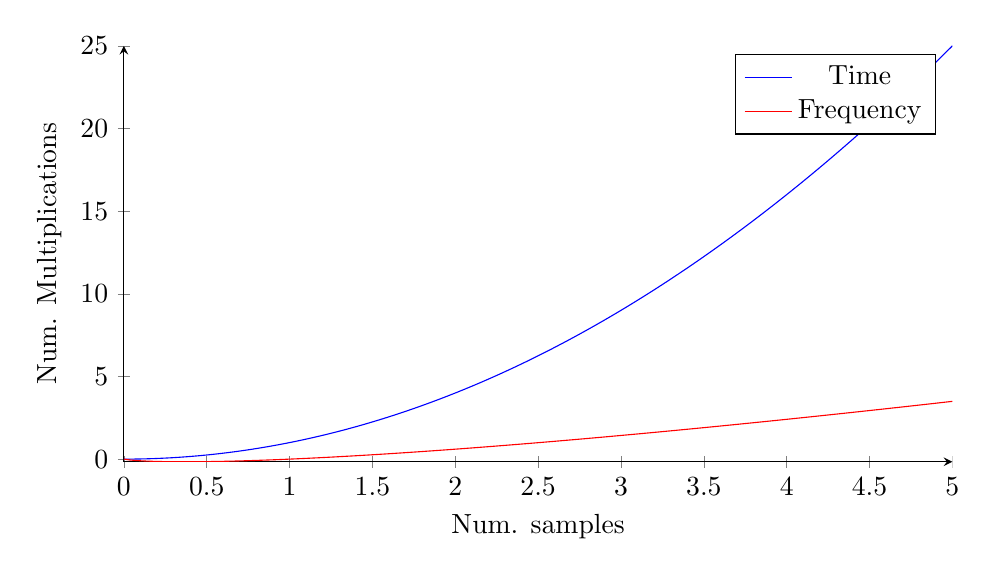
\begin{tikzpicture}
\begin{axis}[
	axis lines = left,
	domain = 0:5,
	samples=150,
	no marks,	
	x post scale=1.25,
	xlabel=Num. samples,
	ylabel=Num. Multiplications,
	y post scale=0.75
]
\addplot {x^2};
\addlegendentry{Time}
\addplot [color=red]{x*(log10(x)))};
\addlegendentry{Frequency}

\end{axis}
\end{tikzpicture} % 
\\ 	



\subsection{Reconstruction with the DAC}
The below figure shows what the previous section accomplished. Our stored discrete signal is convolved with our systems impulse response to filter out the unwanted frequencies, then develop our output waveform. The graph below comes from Nutaq.com's blog posts reviewing the theory and application of analog to digital conversion$^2$.
\\
\begin{center}
\includegraphics[scale=.5]{AtoD_signalsteps}
\end{center}

Notice at the second to bottom, the output waveform is a very choppy waveform that looks like a stitching together of different square waves each at different amplitudes. The primary method to smoothing out this waveform would be to add a low pass filter in between the D/A and the speaker (or other output medium). This will remove the high frequency components made at the edges of the signal. The wikipedia page for \textit{Digital to Analog Converter} provides this image showing both the choppy digital waveform and filtered form.\\ 
\includegraphics[scale=1]{digitalsmoothed}

Another method to improve the waveform would be to  \textbf{oversample} the waveform, which is an umbrella term for interpolating additional points in between the saved points. There are many different ways to interpolate these points such as using a linear curve fit between points to generate more data points. Another more common approach is to calculate the average between two points. The way this is done is by adding zeros in between the points in the frequency domain which creates additional points at the averages between points in the time domain. Some CD players and audio equipment oversample the wave forms to generate a cleaner sound.



% Oversampling for a CD player. Generally the oversampling would be easier to do in the FIR filter. 


\subsection*{Resources}
$^1$ \url{https://en.wikipedia.org/wiki/Digital-to-analog_converter}
$^2$ \url{https://www.nutaq.com/blog/analog-digital-%E2%80%93-part-2-conversion-process}
\part*{Week VII}
\renewcommand\partcontent{Week VII}
%\section*{DAC Transfer Function}

\section{Leakage}
The Fourier transform works only if a specific assumption is made. That assumption being the signal to be transformed is periodic. This proves to be problematic when many signals are non-periodic. \\
\begin{center}
\includegraphics[scale=1]{nonperiodicleakage}
\end{center}
Assuming a non-periodic signal is periodic creates discontinuities in the Fourier Series that adds in many high frequency terms to the sample in the frequency domain. The discontinuities can be seen on the right side of the figure above, highlighted in red. This will decrease the accuracy of our calculations made. Leakage is a common problem faced in signal analysis and while it can't always be completely removed, its effects can be mitigated.


\subsection{Zero Padding}
One simple approach to lessening the effects of leakage is called \textbf{Zero Padding.} This method works best when the sample has a small number of non-zero samples or the sequence and DFT have different lengths. Below is a prime example of how adding additional zeros to the sample can improve the resolution of the signal transform. This example was provided by 	user \textit{Tarin Ziyaee} on the Digital Signal Processing Stack Exchange forum.

\begin{center}
\includegraphics[scale=0.6]{zero_padding}
\end{center}

\subsection{Windowing}
Another common method for dealing with leakage is to multiply the sample in time by a \textbf{windowing function.} This is a function of time that begins and ends at zero, generally increases in intensity at the center, and tapers back out in a common "bell-shaped" curve. Below is a rough example of a windowing function plotted against the original signal in time and its product on the right (not featuring the usual bell shape).
\begin{center}
\includegraphics[scale=0.6]{windowinggraphs_windowed}
\end{center}

Windowing functions are effective in reducing the effects of spectral leakage. They change the distribution of the spectral leakage in different ways which will normally depend on what is needed by the application. There are many popular windowing functions that can be used, yet a very common one is known as the \textbf{Hann Window.} The Hann window is a popular bell-shaped curve that in time follows the function for range $0 \\leq t < \leq N $ with length of window equal to $N+1$ where $N$ can be even or odd. $$w(t) = \frac{1}{2} \bigg[ 1 - cos \bigg( \frac{2\pi t}{N} \bigg) \bigg] = sin^2 \bigg(\frac{\pi t}{N} \bigg) $$ 
Wikimedia Commons hosts this handy image showing a graph of the Hann Window funciton in the time domain and the frequency response of its DFT. 
\begin{center}
\includegraphics[scale=0.3]{hann_window}
\end{center}



\section*{Frequency Translation}
This next section is a departure from the previous sections content yet is another application for using the frequency domain and Fourier transforms. A field which has taken great advantage of signal processing techniques is wireless communication. To communicate wirelessly over radio waves, the frequencies need to be shifted to very high frequencies.
\subsection{Shifting Up}
We want to shift the frequency up to a higher one. This means in the frequency domain our input signal $X(f)$ will need to look like:
$$X(f) \rightarrow X(f-f_c) $$ where $f_c$ is the new frequency our signal is centered at. The best way to find out how this desired $X(f-f_c)$ is derived, we will transform it back to the time domain using the IFT.
$$\mathscr{F}^{-1} [X(f-f_c)]= \int_{-\infty}^{\infty} X(f-f_c)e^{j2\pi ft} df $$ 
A substitution of units will allow us to evaluate this further, so we will declare a new variable, $f'$. 
$$ f'=f-f_c \Rightarrow \quad df' = df \qquad f=f' +f_c $$
Substituting in our new units gives us the following.
$$\rightarrow \int_{-\infty}^{\infty} X(f')e^{j2\pi (f'+f_c)t}df' = e^{j2\pi f_c t} x(t) $$
%The real part of this is what matters to us as performing complex operations outside of a digital system can prove to be difficult.
$$Re\{ e^{j2\pi f_c t} x(t)\} = x(t)cos(2\pi f_c t) $$
This equation gives us a formula to shift the frequency, yet we aren't fully sure yet how transforming just the real part of this signal will look in the frequency domain. We want to avoid complex operations in the time domain as much as possible, so we need to know how it will act in the frequency domain.

$$\mathscr{F} [x(t)cos(2\pi f_c t)] = \int_{-\infty}^{\infty} x(t)cos(2\pi f_c t) e^{-j2\pi f_c t} dt $$

We can simplify cosine into two exponential terms like so.
$$cos(2\pi f_c t) = \frac{e^{j2\pi f_c t}+e^{-j2\pi f_c t}}{2} $$

This gives us a linear sum of two different shifted Fourier transforms, giving the final answer: 
$$\rightarrow 0.5\int_{-\infty}^{\infty} x(t) e^{-j2\pi (f-f_c) t} dt + 0.5\int_{-\infty}^{\infty} x(t) e^{-j2\pi (f+f_c) t} dt $$
$$\Rightarrow \frac{1}{2} X(f-f_c) + \frac{1}{2} X(f+f_c) $$

The below graphic shows our original frequency range centered at zero. The second line shows the new frequency split in half and shifted up/down to $f_c$. Generally this is done to shift audio frequencies up to 15 MHz or higher for wireless transmissions, so do note that the below graph is not drawn to scale but is merely for conceptual illustration.
\begin{center}
\includegraphics[scale=1.65]{freqshiftDrawing_topbit}
\end{center}
Here is a block diagram showing our radio transmission system so far:
\begin{center}
\includegraphics[scale=1]{radioTransmitter}
\end{center}
\textit{Note: The input on the left should be a microphone and it is not pictured, but using a low pass filter is highly recommended between the microphone and mixer}


\subsection{Shifting Down}
Shifting the frequency up can have many uses, yet for the radio transmission and reception analogy, we need to be able to receive. Our fictional antenna can catch and read those signals yet needs to shift them back down to its original range of frequencies for the user to be able to hear the message. Luckily, this can be easily accomplished using the same trick we used prior by mixing the signal with $cos(2\pi f_c t)$. This will split the two new curves we made when shifting up into three new curves. One centered at the original frequency pre-translation, and two new blips centered at $\pm 2 \cdot f_c$. 
\begin{center}
\includegraphics[scale=1]{freqshiftbot}
\end{center}
This adds another need for the low pass filter to ensure those extra high frequency signals don't cause interfence once our signal enters whatever medium we are using for output. This new signal will mathematically have the form of: $$\frac{1}{4} X(f-2f_c) + \frac{1}{2} X(f) + \frac{1}{4} X(f+2f_c) $$
Note the fractional coefficients on each term. While it would be easy to believe these would be a problem, there are many other, much more impactful factors at play in a radio transmission. Much more of that signal strength will be lost to transmission loss then from those coefficients, meaning these fractions are generally ignored. Due to those losses, a very strong amplifier is crucial to performing these transmissions and receptions. Our receiver system as a block diagram looks as such:

\begin{center}
\includegraphics[scale=1]{radioReceiver}
\end{center}


In conclusion, the three frequency plots are laid out below along with our full radio transmission and reception system. 

\begin{center}
\includegraphics[scale=1]{freqshiftDrawing}
\end{center}

\textbf{Final transmitter}
\begin{center}
\includegraphics[scale=0.4]{radioTransmitSystem}
\end{center}


\subsection*{Resources}
\url{https://dsp.stackexchange.com/questions/10293/zero-padding-in-fft} \\
\url{https://commons.wikimedia.org/wiki/File:Window_function_(hann).svg}


\renewcommand\partcontent{Week VIII}
\part*{Week VIII}


\section{Single Side-Band Transmission}
The previous week, we looked at the problem of shifting up a frequency for radio transmission. The solution we derived does create a new problem. Space on radio spectrum is very valuable to allow for other people/agencies to use it and many countries have strict national regulations. Our translated-up frequency is taking twice the room on the frequency spectrum but half of it is a duplicate. We want to cut out that duplicate half. A common method for this is to transmit in \textbf{single sideband} (abbrev. as SSB). To introduce this, we need to talk about some general notation for \textbf{band-pass signals.}

Band-pass is a general term used in many different signals applications yet in this context, it is used to refer to low frequency signals. For our generalized transmitter, the portion of our signal that is band-pass would be the audio signal before it's been translated up for transmission. Many systems will perform some kind of operations and/or filtering on a signal before raising it up for transmission. For notation purposes, we will refer to the input audio as $m(t)$ and the signal after its been processed by the generic system as $g(t)$. From this, we can determine that the signal $g(t)$ will have the form:
$$g(t) = x(t) + j\cdot y(t)$$ 
For transmission to a real antenna, we can't send all of the complex signal $x(t) + jy(t)$.Our output needs to be only the real part (\textit{$v(t)$ will be the signal outputting to the antenna}).
$$v(t)=Re\{ \ g(t)e^{j2\pi f_ct} \ \}$$
$$\rightarrow Re\{ g(t)\} = Re\{\ (x+jy)\ (cos(2\pi f_ct) + jsin(2\pi f_ct))\ \} $$
$$\quad \ = x(t)cos(2\pi f_ct) - y(t)sin(2\pi f_ct)$$
Knowing the form needed for $g(t)$ lets us know that our general system will take the form outlined below.
\begin{center}
\includegraphics[scale=0.75]{BPF_Top}
\end{center}

In the frequency domain, our equations will take the form.
$$\mathscr{F} [g(t)e^{j2\pi f_ct}] = G(f-f_c) $$
$$\mathscr{F} [Re\{ g(t)e^{j2\pi f_ct} \}] = \frac{1}{2}\mathscr{F} [g(t)e^{j2\pi f_ct} + g^*(t)e^{-j2\pi f_ct} ] $$


Now for SSB, we want to get rid of one of those previously mentioned duplicate halves. We want to keep the real part and shift over the imaginary part. For that, we will use the \textbf{Hilbert Transform} which utilizes the $sgn(f)$ function which is equal to: 
\[
    sgn(f)=\left\{
                \begin{array}{ll}
                  1, \quad f \neq 0\\
                  0, \quad f = 0 \\
                \end{array}
              \right.
  \]

The transfer function of $sgn(f)$ is 1:1 on the magnitude plot but will shift the phase by $90^\circ$. This will turn the sinusoidal imaginary component we have into a cosine, allowing us to remove the duplicate half and add it to our real part. We don't want to double or cancel out our signal when it's summed to make $v(t)$, so we will multiply them both by $\frac{1}{2}$. This gives the band-pass filter for SSB transmission a transfer funciton of 
$$u(f) = \frac{1}{2} - \frac{j}{2} sgn(f)$$
Therefore:
$$G(f) = u(f)M(f) = \frac{1}{2}M(f) - \frac{j}{2} sgn(f)M(f)$$
We can model our general transmitter system showing the two separate transfer functions for the real and imaginary parts of $G(f)$.
\begin{center}
\includegraphics[scale=0.75]{BPF_SSB}
\end{center}

Hilbert Transforms have many useful applications, they enable us to easily convert our double side-banded transmission to single. We only need to make a simple change in our equations. An example of how our transmission differs based on the modulation method (double vs single) is plotted below.$^1$ \textit{Note the Full AM modulation would be an example of double side-banded modulation.}\\
\begin{center}
\includegraphics[scale=1]{SSB.png}
\end{center}

\subsection*{Resources}
$^1$\url{https://upload.wikimedia.org/wikipedia/en/thumb/1/1f/SSB_bandform.svg/220px-SSB_bandform.svg.png}


\end{document}